\documentclass{beamer}

%%%%%%%%%%%%%%%%%%%%%%%%%%%%%%%%%%%%%%%%%%%%%%%%%%%%%%%%%%%%%%%%%%%%%%%
% Definicion de paquetes
\usepackage{minted}
\usepackage[utf8]{inputenc}
\usepackage[spanish]{babel}
\usepackage{hyperref}
\usepackage[nodayofweek,level]{datetime}
\usepackage{xargs}
\usepackage[colorinlistoftodos,prependcaption,textsize=tiny]{todonotes}
\presetkeys{todonotes}{inline}{}
\usepackage{pgfpages}

%%%%%%%%%%%%%%%%%%%%%%%%%%%%%%%%%%%%%%%%%%%%%%%%%%%%%%%%%%%%%%%%%%%%%%%
% Definición de comandos
\setlength{\marginparwidth}{2cm}
% \unsure{I'm not sure}
\newcommandx{\unsure}[2][1=]{\todo[linecolor=red,backgroundcolor=red!25,bordercolor=red,#1]{#2}}
% \change{This must be changed}
\newcommandx{\change}[2][1=]{\todo[linecolor=blue,backgroundcolor=blue!25,bordercolor=blue,#1]{#2}}
% \info{Just information}
\newcommandx{\info}[2][1=]{\todo[linecolor=green,backgroundcolor=green!25,bordercolor=green,#1]{#2}}
% \improvement{THIS must be improved}
\newcommandx{\improvement}[2][1=]{\todo[linecolor=orange,backgroundcolor=orange!25,bordercolor=orange,#1]{#2}}
\newcommandx{\thiswillnotshow}[2][1=]{\todo[disable,#1]{#2}}
\newcommand{\mydate}{\formatdate{3}{12}{2021}}

\graphicspath{ {images/} }
%%%%%%%%%%%%%%%%%%%%%%%%%%%%%%%%%%%%%%%%%%%%%%%%%%%%%%%%%%%%%%%%%%%%%%%
% Beamer
\usetheme{Madrid}
\AtBeginEnvironment{minted}{\fontsize{12}{12}\selectfont}
\setbeameroption{show notes on second screen=right}
% \setbeameroption{show only notes}
\setbeameroption{show notes}
% \setbeamertemplate{note page}[default]
%%%%%%%%%%%%%%%%%%%%%%%%%%%%%%%%%%%%%%%%%%%%%%%%%%%%%%%%%%%%%%%%%%%%%%%
% Título
\title[ACFI]{Property-based Testing con PropEr}
\author[M. Ruiz (UCM)]{Miguel Emilio Ruiz Nieto}
\date{\mydate}
%%%%%%%%%%%%%%%%%%%%%%%%%%%%%%%%%%%%%%%%%%%%%%%%%%%%%%%%%%%%%%%%%%%%%%%
%% Empieza el documento
\begin{document}
  \begin{frame}
    \titlepage
  \end{frame}

  \begin{frame}{Contenidos}
    \tableofcontents[hideallsubsections]
  \end{frame}

  \section{Motivación}
    \begin{frame}[fragile]{Motivación}
      \begin{minted}[fontsize=\small]{erlang}
        -module(sort_lib).

        -export([sort/1]).
        % Implementation of quicksort algorithm
        -spec sort(list(integer())) -> list(integer()).
        sort([]) -> [];
        sort([P|Xs]) ->
          sort([X || X <- Xs, X < P]) ++
              [P] ++ sort([X || X <- Xs, P < X]).
      \end{minted}
    \end{frame}

    \begin{frame}[fragile]{Motivación. Test unitarios}
      \begin{minted}[fontsize=\small]{erlang}
        -module(sort_lib_eunit).

        -include_lib("eunit/include/eunit.hrl").

        sort_test_() ->
          [test_zero(), test_two(), test_four()].
        test_zero() ->
            ?_assertEqual([], sort_lib:sort([])).
        test_two() ->
            [?_assertEqual([17,42],
                    sort_lib:sort([X,Y]))
                      || {X,Y} <- [{17,42}, {42,17}]
            ].
        test_four() ->
            ?_assertEqual([1,2,3,4],
                    sort_lib:sort([3,1,4,2])).
      \end{minted}
    \end{frame}

    \begin{frame}{Motivación}
      \begin{block}{Preguntas}
        \begin{itemize}
          \item ¿Son buenos estos tests?
          \item ¿Harían falta más?
          \item En caso de que sí, ¿cuántos más?
        \end{itemize}
      \end{block}
    \end{frame}

    \begin{frame}{Motivación}
      Las metodologías de testing tradicionales son útiles ya que:
      \begin{itemize}
        \item Obliga a los desarrolladores a escribir casos de prueba\\
        del software desarrollado
        \item Para cada input se debe generar un cierto output con el fin\\
        de comprobar el correcto funcionamiento del sistema
      \end{itemize}
    \end{frame}

    \begin{frame}{Motivación}
      Pero tienen sus inconvenientes:
      \begin{itemize}
        \item Consumen tiempo (€€€)
        \item No se garantiza que la batería de tests cubra todos los casos
      \end{itemize}
    \end{frame}

    \begin{frame}{Motivación}
      \begin{exampleblock}{La alternativa}
        \textbf{Property-based testing}
      \end{exampleblock}
    \end{frame}

  \section{Definiciones}
    \begin{frame}{Property-based Testing. Definición}
      \begin{itemize}
        \item Es una técnica para hacer pruebas sobre las propiedades\\
        de nuestro sistema
        \item Los tests no son sobre casos de uso, sino sobre el\\
        comportamiento del propio sistema
        \item Muy común en lenguajes de programación funcional (i.e Quickcheck)
      \end{itemize}
    \end{frame}

    \begin{frame}{Property-based Testing. Definición}
      El proceso de aplicar PBT se divide en dos fases:
      \begin{itemize}
        \pause
        \item Generar datos de entrada de manera aleatoria (Generadores)
        \pause
        \item Hacer verificaciones de las funciones aplicadas a esos datos (Propiedades)
      \end{itemize}
    \end{frame}

    \begin{frame}{Propiedades}
      \begin{itemize}
        \item Son reglas generales que describen el comportamiento de una\\
        función o un programa
        \item Han de ser aplicables a cualquier tipo de entrada y salida del\\
        propio programa bajo sus propias condiciones
        \item La salida debe verificar ciertas características deseadas
      \end{itemize}
    \end{frame}

    \begin{frame}{Propiedades}
      Al principio puede resultar no tan trivial como los tests unitarios ya que:
      \begin{itemize}
        \item El desarrollador ha de tener una visión más nítida de los\\
        casos de uso y del comportamiento del sistema
      \end{itemize}
      No obstante:
      \begin{itemize}
        \item Asegura encontrar un mayor número de ``casos esquina'' y bugs\\
        dentro del código
      \end{itemize}
    \end{frame}

  \section{Erlang}
    \subsection{Historia}
      \begin{frame}{Erlang}
        \begin{itemize}
          \item Lenguaje de programación desarrollado en Ericsson
          \item Orientado a sistemas distribuidos:
          \begin{itemize}
            \item Modelo de actores
            \item Paso de mensajes
            \item Tolerancia a fallos
            \item Alta disponibilidad
            \item Filosofía ``Let it crash''
          \end{itemize}
        \end{itemize}
      \end{frame}

    \subsection{Sintaxis}
      \begin{frame}[fragile]{Sintaxis. Módulos y funciones}
        \begin{minted}{erlang}
          -module(sucessions).
          -export([fib/1]).

          fib(0) -> 0;
          fib(1) -> 1;
          fib(N) -> fib(N-1) + fib(N-2).
        \end{minted}
      \end{frame}

      \begin{frame}[fragile]{Sintaxis. Listas}
        \begin{minted}{erlang}
          1> [First | TheRest] = [1,2,3,4,5].
          2> First.
          1
          3> TheRest.
          [2,3,4,5]
        \end{minted}
      \end{frame}

      \begin{frame}[fragile]{Sintaxis. Tuplas}
        \begin{minted}{erlang}
          4> X = 10, Y = 4.
          4
          5> Point = {X,Y}.
          {10,4}
          6> PreciseTemperature = {celsius, 23.213, 45}.
        \end{minted}
      \end{frame}

      \begin{frame}[fragile]{Sintaxis. Pattern Matching}
        \begin{minted}{erlang}
          is_even(N) when N rem 2 == 0 -> true;
          is_even(_) -> false.
        \end{minted}
      \end{frame}

      \begin{frame}[fragile]{Sintaxis. Funciones de Orden Superior}
        \begin{minted}{erlang}
          7> Add_3 = fun(X) -> X + 3 end.
          #Fun<erl_eval.7.126501267>
          8> lists:map(Add_3, [1,2,3]).
          [4,5,6]
        \end{minted}
      \end{frame}

  \section{PropEr}
    \begin{frame}{PropEr}
      \begin{itemize}
        \item Herramienta para realizar property-based testing en Erlang
        \item Inspirada en Quickcheck
        \item Completamente integrada con los tipos de Erlang
      \end{itemize}
    \end{frame}

    \begin{frame}{PropEr}
      Nos centraremos en los siguientes aspectos:
      \begin{itemize}
        \item Generadores
        \item Estructura de las propiedades
        \item Propiedades sin estado
        \item Propiedades con estado
        \item Reducción de contraejemplos (\textit{shrinking})
      \end{itemize}
    \end{frame}

    \subsection{Generadores}
      \begin{frame}{PropEr. Generadores}
        \begin{itemize}
          \item Funciones que \textit{generan} entradas de una manera ``aleatoria''
          \item Proporcionan datos en base al tipo del generador y a los filtros dados
          \item Pueden ser:
          \begin{itemize}
            \item En base a los tipos de Erlang
            \item Customizados por el desarrollador
          \end{itemize}
        \end{itemize}
      \end{frame}

      \begin{frame}{PropEr. Generadores. Ejemplos}
        Basados en los tipos de Erlang
        \begin{block}{~\vspace{0.7cm}}
          \begin{center}
          \vspace{-0.8cm}
          \begin{tabular}{p{0.45\textwidth}|p{0.45\textwidth}}
            \textcolor{white}{\bf Generador} & \textcolor{white}{\bf Muestra} \\
              \mint{erlang}{integer()} & \mint{erlang}{89234} \\ \hline
              \mint{erlang}{boolean()} & \mint{erlang}{true, false} \\ \hline
              \mint{erlang}{list(Type)} & \mint{erlang}{[true, true, false]} \\ \hline
              \mint{erlang}{tuple()} & \mint{erlang}{{true, 13.321123, -67}} \\
          \end{tabular}
          \end{center}
        \end{block}
      \end{frame}

      \begin{frame}[fragile]{PropEr. Generadores. Ejemplos}
        Customizados por el desarrollador
        \begin{minted}[fontsize=\small]{erlang}
          ?LET(InstanceOfType, TypeGenerator, Transform).
        \end{minted}
        \begin{itemize}
          \item \mintinline{erlang}{InstanceOfType} : La variable que contendrá los datos\\
          generados por el generador del segundo argumento
          \item \mintinline{erlang}{TypeGenerator} : La función generadora que produce los\\
          datos que se almacenan en el argumento anterior
          \item \mintinline{erlang}{Transform} : Expresión que transforma los datos\\
          de la propia función y los acumula en el argumento anterior
        \end{itemize}
      \end{frame}

      \begin{frame}[fragile]{PropEr. Generadores. Ejemplos}
        \begin{minted}[fontsize=\small]{erlang}
          % Customized Generator
          list_no_dupls(T) ->
            ?LET(L, list(T), remove_duplicates(L)).

          % Helper
          remove_duplicates([]) -> [];
          remove_duplicates([A|T]) ->
              case lists:member(A, T) of
                  true -> remove_duplicates(T);
                  false -> [A|remove_duplicates(T)]
              end.
        \end{minted}
      \end{frame}

    \subsection{Estructura de las propiedades}
      \begin{frame}[fragile]{PropEr. Estructura de las propiedades}
        \begin{minted}[fontsize=\small]{erlang}
          ?FORALL(InstanceOfType, TypeGenerator,
            PropertyExpression).
        \end{minted}
        \begin{itemize}
          \item \mintinline{erlang}{InstanceOfType} : La variable que contendrá los datos\\
          generados por los generadores
          \item \mintinline{erlang}{TypeGenerator} : La función generadora que produce los\\
          datos que se almacenan en el argumento anterior
          \item \mintinline{erlang}{PropertyExpression} : Expresión booleana que especifica\\
          la propiedad que se desea verificar
        \end{itemize}
        \note{The data for the test case is generated by the functions\\
          we will enter in the \textbf{TypeGenerator} position, called the generators.
          The framework will take these generators, execute them, and\\
          turn them into actual data, which will then be bound to the\\
          \textbf{InstanceOfType} variable. This variable is then made available\\
          within \textbf{PropertyExpression}, a piece of arbitrary code that must\\
          return true if the test is to pass, or false if it is to fail.\\
          Since \textbf{PropertyExpression} is a single expression, you’ll frequently\\
          see begin ... end blocks used in that area to wrap \\
          more complex sequences of expressions into a single one.}
      \end{frame}

      \begin{frame}[fragile]{PropEr. Estructura de las propiedades. Ejemplos}
        \begin{minted}[fontsize=\small]{erlang}
          -module(prop_sort_lib).

          -include_lib("proper/include/proper.hrl").

          % Propiedad con generador con tipo de Erlang
          prop_same_length() ->
              ?FORALL(L, list(integer()),
                length(L) =:= length(sort_lib:sort(L))).

          % Propiedad con generador customizado
          prop_same_length_no_dupls() ->
              ?FORALL(L, list_no_dupls(integer()),
                length(L) =:= length(sort_lib:sort(L))).
        \end{minted}
      \end{frame}

      \begin{frame}[fragile]{PropEr. Estructura de las propiedades. Ejemplos}
        \begin{minted}[fontsize=\footnotesize]{erlang}
          prop_exists_already_sorted() ->
            ?EXISTS(L, list(integer()), L =:= sort_lib:sort(L)).

          prop_not_exists_different_sorted_after_double_sort() ->
            ?NOT_EXISTS(L, list(integer()),
              sort_lib:sort(L) =/= sort_lib:sort(sort_lib:sort(L))).

        \end{minted}
      \end{frame}

    \subsection{Propiedades con estado}
      \begin{frame}{PropEr. Propiedades con estado}
        \begin{itemize}
          \item Hasta ahora los ejemplos que hemos visto eran \textit{sin estado}
          \item Nos interesa verificar que aquellas aplicaciones que tras realizar
          una operación y cambian su estado mantienen la consistencia
          \item Ideal para los behaviours \mintinline{erlang}{gen_server} y
          \mintinline{erlang}{gen_statem}
        \end{itemize}
      \end{frame}

      \begin{frame}{PropEr. Propiedades con estado}
        \begin{itemize}
          \item Los tests con estado se dividen en dos fases:
          \begin{itemize}
            \item Fase abstracta: se crea el escenario de test (Modelo)
            \item Fase real: El sistema donde se aplican los comandos\\
            generados para dicho modelo
          \end{itemize}
        \end{itemize}
      \end{frame}

      \begin{frame}[plain]{PropEr. Propiedades con estado}
        Fase abstracta

        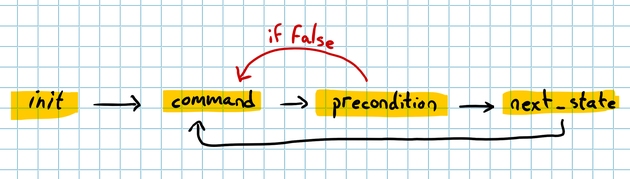
\includegraphics[width=\textwidth]{stateful-symbolic.png}
        \note{In the abstract mode, a command generator creates a symbolic\\
        call with its arguments based on an initial model state. PropEr\\
        then applies the preconditions to that command to know if it would\\
        be valid. If the validation fails, PropEr tries again with a new\\
        generated command. Once a suitable command is found, we can move\\
        forward. The next\_state function takes the command and the current\\
        state, and has to return a new state data structure. Then the whole\\
        process is repeated over and over, until PropEr decides it has enough\\
        commands.}

      \end{frame}

      \begin{frame}{PropEr. Propiedades con estado}
        Fase real
        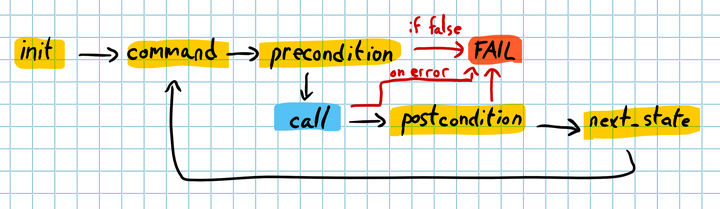
\includegraphics[width=\textwidth]{stateful-actual-bw.png}
        \note{The execution is repeated, except that now, at every step of the way,\\
        PropEr also runs the commands against the real system. The preconditions\\
        are still reevaluated to ensure consistency so that if a generated precondition\\
        that used to work suddenly fails, the entire test also fails. The next symbolic\\
        call in the list is executed, with its result stored. The postcondition is then\\
        evaluated, and if it succeeds, the state transition for the command is applied\\
        to the state and the next command can be processed.

        In case of a failure, shrinking is done by modifying the command sequence as\\
        required, mostly by removing operations and seeing if things still work.\\
        Preconditions will be used by the framework to make sure that the various\\
        attempts are valid.}
      \end{frame}

    \subsection{Shrinking}
      \begin{frame}{PropEr. Reducción de contraejemplos}
        \begin{itemize}
          \item En algunos casos, puede haber ciertos tests que no\\
          cumplan las propiedades que hemos definido
          \item PropEr es capaz de aplicar \textit{reducciones} hasta llegar\\
          al contraejemplo más pequeño posible
        \end{itemize}
      \end{frame}

      \begin{frame}[fragile]{PropEr. Reducción de contraejemplos}
        \begin{minted}{shell}
          ~ $ rebar3 proper
          ===> Verifying dependencies...
          ===> Compiling sort_lib
          ===> Testing prop_sort_lib:prop_same_length()
          .........!
          Failed: After 10 test(s).
          [9,-2,8,-2]

          Shrinking ..(2 time(s))
          [-2,-2]
          ===>
          0/1 properties passed, 1 failed
          ===> Failed test cases:
          prop_sort_lib:prop_same_length() -> false
        \end{minted}
      \end{frame}

  \section{Un caso real}
    \begin{frame}{Un caso real}
      \begin{itemize}
        \item Coowry. Empresa dedicada a los pagos a través de \textit{airtime}
        \item Cientos de clientes diariamente realizaban pagos a través del API
        \begin{itemize}
          \item El formato de las transacciones no siempre era el mismo
          \item Caídas de servicio
        \end{itemize}
        \pause
        \begin{exampleblock}{La solución}
          Baleen. Biblioteca de validadores escritos en Erlang
        \end{exampleblock}
      \end{itemize}
    \end{frame}

    \begin{frame}[fragile]{Baleen. Tipos}
      \begin{minted}[fontsize=\small]{erlang}
        -type validator(A, B) :: (fun(A) -> result(B) end).
        -type result(A) :: {ok, A} | {error, binary()}.
        -type str() :: string() | binary().

        -spec validate(validator(A,B), A) -> result(B).
        %% @doc Validates data with a validator.
        %% `X' is the term to be validated with
        %% validator `V'.
        validate(V, X) -> V(X).
      \end{minted}
    \end{frame}

    \begin{frame}[fragile]{Baleen. Validadores}
      \begin{minted}[fontsize=\small]{erlang}
        -spec valid() -> validator(_,_).
        %% @doc Returns a validator that always validates.
        valid() ->
          fun(X) -> {ok, X} end.
      \end{minted}
    \end{frame}

    \begin{frame}[fragile]{Baleen. Validadores}
      \begin{minted}[fontsize=\footnotesize]{erlang}
        -spec to_integer() -> validator(str(), integer()).
        %% @doc Returns a validator that takes a `Value'
        %% and tries to cast to integer. If the cast success,
        %% `{ok, Integer}' is returned, otherwise,
        %% `{error, <<"Value is not an integer">>}' is returned.
        to_integer() ->
          fun(Value) when is_binary(Value)->
              try erlang:binary_to_integer(Value) of
                Integer -> {ok, Integer}
              catch
                _:_ -> {error, format("~p is not an integer", [Value])}
              end;
             (Value) ->
              case io_lib:fread("~d",Value) of
                {ok, [Integer], []} -> {ok, Integer};
                _ -> {error, format("~p is not an integer", [Value])}
              end
          end.
      \end{minted}
    \end{frame}

    \begin{frame}[fragile]{Baleen. Tests en PropEr}
      \begin{minted}[fontsize=\footnotesize]{erlang}
        prop_valid() ->
          ?FORALL(Data, term(),
            begin
              {ok, Data} == baleen:validate(valid(), Data)
            end).

        prop_is_integer_with_integer_strings() ->
        ?FORALL(Integer, integer(),
                {ok, Integer} == baleen:validate(to_integer(),
                                          integer_to_list(Integer))).

        prop_is_integer_with_integer_binaries() ->
          ?FORALL(Integer, integer(),
                  {ok, Integer} == baleen:validate(to_integer(),
                                          integer_to_binary(Integer))).
      \end{minted}
    \end{frame}

  \section{Conclusiones}
    \begin{frame}{Conclusiones}
      \begin{itemize}
        \item Merece la pena usar PBT porque es capaz de generar casos de test muy `rápido'
        \item No obstante,
        \begin{itemize}
          \item Hay casos en los que puede merecer la pena más hacer test unitarios
          \item A veces cuesta más definir las propiedades que el desarrollo
          pedido.
          \item Se usa poco dado que está muy centrado en lenguajes funcionales
        \end{itemize}
      \end{itemize}
    \end{frame}

  \section{Bibliografía}
    \begin{frame}{Bibliografía}
      \begin{itemize}
        \item Getting Started with Erlang \url{https://www.erlang.org/doc/getting_started/intro.html}
        \item PropEr Guide \url{https://proper-testing.github.io}
        \item Property-Based Testing with PropEr, Erlang and Elixir \url{https://www.propertesting.com/}
        \item Baleen repo \url{https://github.com/coowry/baleen}
      \end{itemize}
    \end{frame}
\end{document}